\documentclass[12pt,a4paper]{elsarticle}

% ===================== METADATOS ESPECÍFICOS DE INF-001 (REV1) =====================
% Se definen ANTES de config/preamble.tex; config/datos_proyecto.tex usa
% \providecommand, de modo que estos valores prevalecen solo en este documento.
\newcommand{\projecttitle}{DISEÑO DEL SISTEMA DE VENTILACIÓN DEL LABORATORIO}
\newcommand{\docRevision}{1}
\newcommand{\docFecha}{27/07/2026}
\newcommand{\docFechaLarga}{27 de julio de 2026}
\newcommand{\fechaRevUno}{27/07/2026}
\newcommand{\descRevUno}{Cambio de alcance del cliente: sistema sin presurización, ventilador axial, sin instrumentación de presión diferencial}

% ===================== IMPORTAR CONFIGURACIÓN MODULAR =====================
% ===================== CONFIGURACIÓN DE PÁGINA =====================
\pdfminorversion=7
\usepackage[top=4.5cm, bottom=2.5cm, left=2.0cm, right=2.0cm,
headheight=4cm, headsep=0.5cm]{geometry}

% ===================== TIPOGRAFÍA Y CODIFICACIÓN =====================
\usepackage[utf8]{inputenc}
\usepackage[T1]{fontenc}
\usepackage[spanish,es-tabla]{babel}
\usepackage{tgtermes}
\usepackage{microtype}

% ===================== SANGRÍAS Y ESPACIADO =====================
\setlength{\parindent}{0pt}
\setlength{\parskip}{6pt}

% ===================== TÍTULOS =====================
\usepackage{titlesec}
\titleformat{\section}{\bfseries\fontsize{12}{14}\selectfont}{\thesection}{1em}{}
\titleformat{\subsection}{\bfseries\fontsize{12}{14}\selectfont}{\thesubsection}{1em}{}
\titleformat{\subsubsection}{\bfseries\fontsize{12}{14}\selectfont}{\thesubsubsection}{1em}{}

% ===================== MATEMÁTICAS =====================
\usepackage{amsmath,amssymb,amsfonts,mathtools}
\usepackage{textgreek,gensymb,siunitx}

% ===================== QUÍMICA Y SÍMBOLOS =====================
\usepackage[version=4]{mhchem}
\usepackage{chemfig,textcomp}

% ===================== COLOR (una sola carga, con soporte de tablas) =====================
\usepackage[table]{xcolor} % Carga colortbl; necesario para \rowcolor

% ===================== TABLAS Y FIGURAS =====================
\usepackage{booktabs,array,longtable,multirow,tabularx}
\usepackage{graphicx,float,subcaption}

% ===================== OTROS PAQUETES =====================
\usepackage{enumitem,listings,algorithm,algpseudocode}
\usepackage{tocloft}
\usepackage{appendix}
\usepackage{eso-pic}
\usepackage{lastpage}

% ===================== ENLACES E HIPERVÍNCULOS (cargar cerca del final) =====================
\usepackage{xurl}
\usepackage[colorlinks=true,linkcolor=blue,citecolor=blue,urlcolor=blue,breaklinks=true]{hyperref}

% ===================== ENCABEZADO CORPORATIVO =====================
\usepackage{fancyhdr}

% ===================== INFORMACIÓN DEL DOCUMENTO =====================
% ===================== DATOS DEL PROYECTO =====================
% Toda la información del proyecto se centraliza aquí para facilitar
% la creación de nuevos informes sin alterar el código fuente.

% 1. Información General del Proyecto
\providecommand{\projecttitle}{DISEÑO DEL SISTEMA DE VENTILACIÓN Y PRESURIZACIÓN DEL LABORATORIO}
\providecommand{\projectnumber}{P2437}
\providecommand{\documentcode}{P2437-HV-INF-001}
\providecommand{\documenttype}{MEMORIA DESCRIPTIVA}
\providecommand{\targetcompany}{BRINSA}

% 2. Información de Documento y Emisión
\providecommand{\docRevision}{1}
\providecommand{\docFecha}{10/09/2026}
\providecommand{\docFechaLarga}{10 de septiembre de 2026}

% 3. Integrantes y Control de Firmas
\providecommand{\firmaElaboro}{J. Arboleda}
\providecommand{\firmaReviso}{H. Rosero}
\providecommand{\firmaAprobo}{F. Navia}

% 4. Fechas de Firmas y Revisiones
\providecommand{\fechaElaboro}{10/09/2026}
\providecommand{\fechaReviso}{10/09/2026}
\providecommand{\fechaAprobo}{10/09/2026}

% 5. Espaciado de la portada (parametrizable por documento)
\providecommand{\portadaVspaceA}{2cm}   % espacio superior
\providecommand{\portadaVspaceB}{2cm}   % espacio antes de las tablas de datos

% 6. Datos de Historial de Revisiones (Portada / Firmas)
% Revisión vigente: REV1 (reubicación de rejillas de exfiltración, CFD actualizado).
\providecommand{\fechaRevCero}{15/07/2026}
\providecommand{\descRevCero}{Emisión inicial}
\providecommand{\fechaRevUno}{10/09/2026}
\providecommand{\descRevUno}{Reubicación de las rejillas de exfiltración (apiladas verticalmente en la pared opuesta a la inyección, disposición BRINSA) y actualización de la simulación CFD y su análisis}


% Adaptaciones para el encabezado corporativo
\newcommand{\documentrevision}{REV \docRevision}
\newcommand{\documentdate}{\docFechaLarga}
\newcommand{\elaboratedby}{\MakeUppercase{\firmaElaboro}}
\newcommand{\reviewedby}{\MakeUppercase{\firmaReviso}}
\newcommand{\approvedby}{\MakeUppercase{\firmaAprobo}}

% ===================== AUTO-NUMERACIÓN DE TABLAS =====================
\newcounter{itemcount}
\newcolumntype{N}{>{\stepcounter{itemcount}\theitemcount}c}

% ===================== CONFIGURACIÓN DE LISTINGS =====================
\lstset{
	basicstyle=\footnotesize\ttfamily,
	breaklines=true,
	frame=single,
	language=Python,
	showstringspaces=false
}

\journal{Revista de Ingeniería}

\input{config/header.tex}

\journal{Revista de Ingeniería}

\begin{document}

% ===================== IMPORTAR SECCIONES MODULARES =====================
\input{sections/00_hojafirmas.tex}
\input{sections/00_portada.tex}

% ===================== NOTA DE REVISIÓN =====================
\section*{Nota de Revisión}
\addcontentsline{toc}{section}{Nota de Revisión}

REV1 (27/07/2026) --- cambio de alcance del cliente: sistema sin presurización, ventilador axial, sin instrumentación de presión diferencial; se mantienen caudal, filtración y rejillas.

\newpage

% ===================== RESTAURAR ESTILO ANTES DEL FRONTMATTER =====================
\pagestyle{corporativo}

% ===================== FRONTMATTER CON MEMBRETE FORZADO =====================
\begin{frontmatter}

	\title{\projecttitle}

	\author[inst1]{J.Arboleda\corref{cor1}}
	\ead{proyectos2@dmlsas.com}

	\author[inst1]{F. Navia}
	\ead{fernando.navia@dmlsas.com}

	\author[inst2]{H. Rosero}
	\ead{herminsul.rosero@dmlsas.com}

	\cortext[cor1]{Autor correspondiente}
	\address[inst1]{DML Ingenieros consultores, Cali, Colombia, 760025}
	\address[inst2]{Especialidad Mecánica y Procesos, Cali, Colombia}

	% ===================== ABSTRACT CON MEMBRETE GARANTIZADO =====================
	\begin{abstract}
		\thispagestyle{corporativo}
		El presente informe técnico describe el diseño conceptual del sistema de ventilación con filtración para un laboratorio de 320 m$^3$ de volumen efectivo. El objetivo consiste en garantizar 12 renovaciones de aire por hora y diluir los contaminantes generados en el interior, con impulsión de aire filtrado y descarga libre a la atmósfera a través de rejillas.

		La estrategia de diseño seleccionada emplea un ventilador axial mural (placa mural) Ø560 mm en PRFV de transmisión directa (sin ductos), uniforme con el montaje típico de la planta, que introduce aire filtrado al recinto, complementado con tres rejillas de descarga libre que permiten la salida ordenada del flujo. Se presentan los cálculos de caudal (2 260 CFM), potencia del ventilador (0.320 kW teórico a 165 Pa en el sitio, motor provisional de 0.75 HP), velocidad real en boca (4.33 m/s a Ø560 mm) y dimensiones de las rejillas de salida (353 mm $\times$ 336 mm cada una, velocidad de descarga 3.0 m/s). Los resultados se sustentan en ASHRAE 170, ASHRAE 62.1, NFPA 99, OSHA 29 CFR 1910.1450, WHO Laboratory Biosafety Manual y NIH DRM.
	\end{abstract}

	\begin{keyword}
		ventilación de laboratorios \sep filtración MERV \sep renovaciones de aire \sep CFD \sep ASHRAE 170 \sep calidad del aire interior
	\end{keyword}

\end{frontmatter}

% ===================== RESTAURAR ESTILO DESPUÉS DEL FRONTMATTER =====================
\pagestyle{corporativo}
\thispagestyle{corporativo}

% ===================== RESUMEN EJECUTIVO =====================
\newpage
\section*{Resumen Ejecutivo}
\addcontentsline{toc}{section}{Resumen Ejecutivo}

El laboratorio objeto de estudio requiere un sistema de ventilación que garantice 12 renovaciones de aire por hora y una presión positiva controlada respecto a los espacios circundantes. La presurización positiva se logra mediante la inyección de aire limpio y filtrado a un caudal superior al de extracción, de modo que el flujo neto se dirija desde el interior hacia el exterior a través de aberturas controladas.

La solución de diseño propuesta utiliza un ventilador de impulsión directa ubicado en una pared del recinto, sin ductos de distribución. El aire ingresa al laboratorio a través de una boca circular equivalente a 412 mm de diámetro (radio 206.0 mm) y a una velocidad de 8 m/s. La salida del aire se efectúa mediante tres rejillas de exfiltración rectangulares de 353 mm $\times$ 336 mm cada una, operando a una velocidad facial de 3.0 m/s.

Los resultados principales indican un caudal de diseño de 64.0 m$^3$/min (3 840 m$^3$/h, 2 260 CFM), una potencia teórica del ventilador de 0.338 kW a las condiciones del sitio (Cajicá, $\rho$ = 0.88 kg/m$^3$) y una potencia instalada recomendada de 1.0 HP. El diseño cumple con los rangos de renovaciones de aire establecidos por ASHRAE 170, WHO y NIH para laboratorios de control medio y bioseguridad nivel 2. Los datos de contorno obtenidos son aplicables de manera directa a un modelo de dinámica de fluidos computacional (CFD) para la verificación del campo de presiones y la distribución de velocidades dentro del recinto.

\newpage

% ===================== NOMENCLATURA =====================
\section*{Nomenclatura y Abreviaturas}
\addcontentsline{toc}{section}{Nomenclatura y Abreviaturas}

\subsection*{Símbolos}
\begin{tabularx}{\textwidth}{@{}lX@{}}
	\toprule
	\textbf{Símbolo} & \textbf{Descripción} \\
	\midrule
	$A$ & Área (m$^2$) \\
	$D$ & Diámetro (m) \\
	$N$ & Número de renovaciones de aire por hora (ren/h) \\
	$P$ & Potencia (kW) \\
	$Q$ & Caudal volumétrico (m$^3$/min o m$^3$/s) \\
	$r$ & Radio (m) \\
	$V$ & Volumen efectivo del recinto (m$^3$) \\
	$v$ & Velocidad (m/s) \\
	$\Delta P$ & Presión diferencial (Pa) \\
	$\eta$ & Eficiencia del ventilador (-) \\
	$\pi$ & Constante matemática (3.14159) \\
	\bottomrule
\end{tabularx}

\vspace{1cm}

\subsection*{Abreviaturas}
\begin{tabularx}{\textwidth}{@{}lX@{}}
	\toprule
	\textbf{Abreviatura} & \textbf{Significado} \\
	\midrule
	ACH & Air Changes per Hour (renovaciones de aire por hora) \\
	ASHRAE & American Society of Heating, Refrigerating and Air-Conditioning Engineers \\
	CFD & Computational Fluid Dynamics \\
	CFM & Cubic Feet per Minute \\
	HEPA & High Efficiency Particulate Air \\
	MERV & Minimum Efficiency Reporting Value \\
	NFPA & National Fire Protection Association \\
	NIH & National Institutes of Health \\
	OSHA & Occupational Safety and Health Administration \\
	WHO & World Health Organization \\
	\bottomrule
\end{tabularx}

\newpage


% ===================== ÍNDICES CON MEMBRETE =====================
\tableofcontents
\listoftables
\listoffigures
\newpage

% ===================== CONTENIDO PRINCIPAL =====================
\section{Introducción}

El control de la calidad del aire interior en laboratorios constituye un requisito crítico para garantizar la integridad de los procesos, la seguridad del personal y la confiabilidad de los resultados analíticos. En instalaciones sensibles a contaminación por partículas o microorganismos, la ventilación debe cumplir simultáneamente dos funciones: diluir contaminantes generados en el interior y evitar la infiltración de agentes externos. La presurización positiva respecto a zonas adyacentes constituye la estrategia más eficaz para alcanzar el segundo objetivo.

El presente informe aborda el diseño conceptual del sistema de ventilación y presurización de un laboratorio con volumen efectivo de 320 m$^3$, ubicado en las instalaciones de BRINSA. El recinto requiere 12 renovaciones de aire por hora, valor seleccionado con base en los estándares internacionales aplicables a laboratorios de control medio y bioseguridad nivel 2. El aire de impulsión se introduce mediante un ventilador directo, sin ductos de distribución, y sale del recinto a través de tres rejillas de exfiltración controladas. Esta configuración minimiza la complejidad constructiva y facilita la modelación posterior mediante dinámica de fluidos computacional (CFD).

El documento se estructura de la siguiente manera. La Sección 2 presenta los objetivos y el alcance del estudio. La Sección 3 define las bases de diseño, incluyendo condiciones ambientales, criterios de ventilación y normativa aplicable. La Sección 4 describe la metodología de cálculo. La Sección 5 presenta los resultados de caudal, potencia, áreas de impulsión y exfiltración, y los datos para CFD. La Sección 6 analiza la coherencia de los resultados con los requerimientos de presurización. Finalmente, las Secciones 7 y 8 presentan conclusiones y recomendaciones.

\section{Objetivos del Proyecto}

\subsection{Objetivo General}

Diseñar el sistema de ventilación y presurización positiva del laboratorio de 320 m$^3$ de volumen efectivo, garantizando 12 renovaciones de aire por hora y evitando la infiltración de contaminantes desde zonas adyacentes.

\subsection{Objetivos Específicos}

\begin{enumerate}
	\item Determinar el caudal de aire de impulsión requerido para alcanzar las 12 renovaciones de aire por hora en el recinto.
	\item Calcular la potencia del ventilador necesaria para vencer las pérdidas de presión del sistema de impulsión y exfiltración.
	\item Dimensionar el área de impulsión del ventilador (configuración circular) y las rejillas de exfiltración rectangulares.
	\item Sustentar el número de renovaciones de aire con base en la normativa internacional aplicable (ASHRAE, WHO, NIH, OSHA, NFPA).
	\item Generar los datos de contorno para un modelo CFD que permita verificar la distribución de velocidades y el campo de presiones en el laboratorio.
\end{enumerate}

\section{Alcance y Limitaciones}

\subsection{Alcance}

El presente informe incluye la definición de las bases de diseño, el cálculo del caudal de ventilación, la estimación de la potencia del ventilador, el dimensionamiento del área de impulsión y de las rejillas de exfiltración, la sustentación normativa de las 12 renovaciones de aire por hora, y la generación de datos de contorno para un modelo CFD. Adicionalmente, se presentan recomendaciones para el control de presión diferencial, la filtración del aire de impulsión y la estanqueidad del recinto.

\subsection{Limitaciones}

El estudio se limita al diseño conceptual del sistema de ventilación y presurización. No se incluye el diseño detallado de ductos, ya que la estrategia seleccionada emplea impulsión directa. No se realiza la selección comercial de un ventilador específico, aunque se indican los parámetros mínimos requeridos. El modelo CFD se ejecutó en Autodesk CFD con las condiciones de contorno presentadas en la Tabla \ref{tab:cfd_boundaries}; los resultados se discuten en las Secciones \ref{sec:resultados} y \ref{sec:analisis}. Las propiedades del aire se consideran aproximadamente constantes a 25 $^{\circ}$C y 101.3 kPa.

\section{Bases de Diseño}

\subsection{Condiciones Ambientales del Sitio}

Las condiciones ambientales del sitio se presentan en la Tabla \ref{tab:environmental_conditions}. Estos valores corresponden a las condiciones del sitio de instalación en Cajicá, Cundinamarca (planta BRINSA) \cite{dml_informe_investigacion_2026} y se utilizan para la estimación de las propiedades del aire de impulsión.

\begin{table}[htbp]
	\centering
	\caption{Condiciones ambientales del sitio de instalación}
	\label{tab:environmental_conditions}
	\setcounter{itemcount}{0}
	\begin{tabularx}{\textwidth}{@{}NXclc@{}}
		\toprule
		\multicolumn{1}{c}{\textbf{Item}} & \textbf{Parámetro Ambiental} & \textbf{Valor} & \textbf{Unidad} & \textbf{Referencia} \\
		\midrule
		& Temperatura ambiente máxima & 21.0 & $^{\circ}$C & IDEAM 2023 \\
		& Temperatura ambiente mínima & 3.0 & $^{\circ}$C & IDEAM 2023 \\
		& Temperatura ambiente promedio & 14.0 & $^{\circ}$C & IDEAM 2023 \\
		& Humedad relativa promedio & 84.0 & \% & IDEAM 2023 \\
		& Presión atmosférica & 74.1 & kPa & NOAA 2022 \\
		& Altitud sobre el nivel del mar & 2 558 & msnm & IGAC 2021 \\
		\bottomrule
	\end{tabularx}
\end{table}

\subsection{Propiedades del Aire de Impulsión}

El aire de impulsión se considera a 21 $^{\circ}$C (condición de diseño de verano 0.4 \%) y 74.1 kPa (condiciones del sitio), con propiedades aproximadas presentadas en la Tabla \ref{tab:air_properties}.

\begin{table}[htbp]
	\centering
	\caption{Propiedades del aire de impulsión}
	\label{tab:air_properties}
	\setcounter{itemcount}{0}
	\begin{tabularx}{\textwidth}{@{}NXclc@{}}
		\toprule
		\multicolumn{1}{c}{\textbf{Item}} & \textbf{Propiedad} & \textbf{Valor} & \textbf{Unidad} & \textbf{Referencia} \\
		\midrule
		& Densidad & 0.88 & kg/m$^3$ & Gas ideal a condiciones del sitio \\
		& Viscosidad dinámica & $1.81 \times 10^{-5}$ & Pa$\cdot$s & Cengel \& Ghajar (2020) \\
		& Temperatura de impulsión & 14.0 & $^{\circ}$C & Criterio de diseño \\
		& Calidad de filtración mínima & MERV 13-14 & -- & ASHRAE 52.2 \\
		\bottomrule
	\end{tabularx}
\end{table}

\subsection{Datos del Recinto y Criterios de Ventilación}

La Tabla \ref{tab:room_data} resume las características geométricas y los criterios de ventilación del laboratorio. El laboratorio se ubica dentro de una planta de hipoclorito de calcio, cuyo ambiente exterior es altamente corrosivo; el ventilador, las rejillas y los soportes expuestos deben ser en PRFV, acero inoxidable 316 o acero con recubrimiento epóxico, y el motor debe ser TEFC anticorrosivo.

\begin{table}[htbp]
	\centering
	\caption{Datos del recinto y criterios de ventilación}
	\label{tab:room_data}
	\setcounter{itemcount}{0}
	\begin{tabularx}{\textwidth}{@{}N>{\hsize=0.9\hsize}X>{\hsize=1.2\hsize}Xc>{\hsize=0.9\hsize}X@{}}
		\toprule
		\multicolumn{1}{c}{\textbf{Item}} & \textbf{Parámetro} & \textbf{Valor} & \textbf{Unidad} & \textbf{Referencia} \\
		\midrule
		& Volumen efectivo del laboratorio & 320 & m$^3$ & Medición / modelo 3D \\
		& Renovaciones de aire requeridas & 12 & ren/h & ASHRAE 170 / WHO / NIH \\
		& Caudal de diseño & 3 840 (64.0 m$^3$/min; 2 260 CFM) & m$^3$/h & Memoria de cálculo \\
		& Estrategia de ventilación & Ventilador directo + rejillas de descarga libre & -- & Criterio de diseño \\
		& Descarga de rejillas & Libre a la atmósfera (sin contrapresión) & -- & Criterio de diseño \\
		\bottomrule
	\end{tabularx}
\end{table}

\subsection{Criterios de Diseño del Ventilador}

La Tabla \ref{tab:fan_criteria} presenta los criterios de diseño del ventilador de impulsión, de tipo axial mural (placa mural) Ø560 mm con transmisión directa, configuración uniforme con el montaje típico instalado en la planta (cubierta intemperie con banco de filtración, estructura de unión pernada al muro y malla de protección interior); el motor va en el cubo del impulsor dentro de la corriente de aire, en ejecución encapsulada severe duty anticorrosiva. El punto de trabajo en el sitio corresponde al escenario de filtración cargada ($\Delta P$ filtro 154 Pa + 11 Pa de pérdida en las rejillas de descarga libre = 165 Pa total); dado que las curvas de catálogo se publican a densidad estándar ($\rho$ = 1.2 kg/m$^3$), la selección comercial se realiza en el punto equivalente de catálogo 3 840 m$^3$/h a 225 Pa \cite{dml_informe_investigacion_2026,dml_hd_vent_001}.

\begin{table}[htbp]
	\centering
	\caption{Criterios de diseño del ventilador de impulsión}
	\label{tab:fan_criteria}
	\setcounter{itemcount}{0}
	\begin{tabularx}{\textwidth}{@{}N>{\hsize=0.9\hsize}X>{\hsize=1.2\hsize}Xc>{\hsize=0.9\hsize}X@{}}
		\toprule
		\multicolumn{1}{c}{\textbf{Item}} & \textbf{Parámetro} & \textbf{Valor} & \textbf{Unidad} & \textbf{Referencia} \\
		\midrule
		& Tipo de ventilador & Axial mural (placa mural) Ø560 mm PRFV/epóxico, transmisión directa (uniformidad con montaje típico de planta) & -- & Criterio de diseño \\
		& Caudal de diseño & 3 840 (1.0667 m$^3$/s) & m$^3$/h & Memoria de cálculo \\
		& Presión total en el sitio (filtro cargado) & 165 & Pa & Memoria de cálculo \\
		& Punto equivalente de catálogo ($\rho$ = 1.2 kg/m$^3$) & 225 & Pa & Corrección de densidad, $k$ = 0.733 \\
		& Presión total en el sitio (filtro limpio) & 70 & Pa & Memoria de cálculo \\
		& Punto equivalente de catálogo (limpio) & 95 & Pa & Corrección de densidad, $k$ = 0.733 \\
		& Eficiencia total supuesta & 0.55 & -- & Criterio de diseño (provisional) \\
		& Potencia teórica de aire & 0.320 (0.43 HP) & kW & Ec. (\ref{eq:potencia}) \\
		& Motor provisional & 0.75 HP TEFC encapsulado anticorrosivo (en la corriente de aire), 440 V, 3$\phi$, 60 Hz (margen de servicio 1.5, a confirmar con catálogo) & -- & Criterio de diseño / cliente \\
		& Diámetro del impulsor (seleccionado) & 560 & mm & Uniformidad montaje típico de planta (REV2) \\
		& Velocidad real en boca (Ø560 mm) & 4.33 & m/s & $Q$ / $A_\text{boca}$ \\
		& Velocidad de impulsión (BC del CFD, histórica) & 8.0 & m/s & Criterio de diseño CFD \\
		& Área de boca de impulsión (BC del CFD, histórica) & 0.1333 & m$^2$ & Ec. (\ref{eq:area_vent}) \\
		& Diámetro equivalente (radio) (BC del CFD, histórica) & 412 (206.0) & mm & Ec. (\ref{eq:diametro}) \\
		\bottomrule
	\end{tabularx}
\end{table}

\subsection{Escenarios de Filtración}

La calidad de filtración definitiva es MERV 13-14: el laboratorio es de análisis industrial y no de biocontención, por lo que la filtración HEPA quedó evaluada y descartada. La Tabla \ref{tab:filtration_scenarios} presenta los escenarios de filtración considerados en el diseño, con las caídas de presión corregidas a la densidad del sitio.

\begin{table}[htbp]
	\centering
	\caption{Escenarios de filtración del sistema de impulsión}
	\label{tab:filtration_scenarios}
	\setcounter{itemcount}{0}
	\begin{tabularx}{\textwidth}{@{}NXcccc@{}}
		\toprule
		\multicolumn{1}{c}{\textbf{Item}} & \textbf{Escenario} & \textbf{$\Delta P$ Filtro} & \textbf{$\Delta P$ Total} & \textbf{Potencia} & \textbf{Estado} \\
		& & \textbf{(Pa)} & \textbf{(Pa)} & \textbf{(kW)} & \\
		\midrule
		& MERV 13-14 limpio & 59 & 70 & 0.136 & Operación inicial \\
		& MERV 13-14 cargado (diseño) & 154 & 165 & 0.320 & Punto de selección \\
		& HEPA H13 limpio & 250 & 261 & 0.506 & Referencia histórica (no aplica) \\
		& HEPA H13 cargado & 600 & 611 & 1.185 & Referencia histórica (no aplica) \\
		\bottomrule
	\end{tabularx}
\end{table}

\subsection{Rejillas de Exfiltración}

La Tabla \ref{tab:grille_criteria} presenta los criterios de diseño de las rejillas de descarga. Las rejillas descargan libremente a la atmósfera: a la densidad del sitio, el cierre de orificio ($C_d$ = 0.60) de las tres rejillas a 3.0 m/s representa una pérdida de descarga de 11 Pa, sin set-point de presión en el recinto \cite{dml_hd_rej_001}.

\begin{table}[htbp]
	\centering
	\caption{Criterios de diseño de las rejillas de exfiltración}
	\label{tab:grille_criteria}
	\setcounter{itemcount}{0}
	\begin{tabularx}{\textwidth}{@{}N>{\hsize=0.9\hsize}X>{\hsize=1.2\hsize}Xc>{\hsize=0.9\hsize}X@{}}
		\toprule
		\multicolumn{1}{c}{\textbf{Item}} & \textbf{Parámetro} & \textbf{Valor} & \textbf{Unidad} & \textbf{Referencia} \\
		\midrule
		& Número de rejillas & 3 & unidades & Criterio de diseño \\
		& Dimensiones por rejilla & 353 $\times$ 336 & mm & Memoria de cálculo \\
		& Velocidad facial & 3.0 & m/s & Criterio de diseño \\
		& Área neta total (por rejilla) & 0.3556 (0.1185) & m$^2$ & Ec. (\ref{eq:area_exfil}) \\
		& Presión de descarga libre ($C_d$ = 0.60) & 11 & Pa & Cierre de orificio, $\rho$ = 0.88 kg/m$^3$ \\
		& Malla anti-insectos & Inox 316, 18$\times$18 (abertura $\approx$1 mm) & -- & Criterio de diseño \\
		\bottomrule
	\end{tabularx}
\end{table}

\subsection{Corrosividad del Ambiente y Criterio de Materiales}

El laboratorio se ubica dentro de una planta de hipoclorito de calcio, cuyo ambiente exterior es altamente corrosivo (cloro, hipoclorito y humedad alta). La Tabla \ref{tab:material_criteria} resume el criterio de materiales adoptado para los componentes expuestos \cite{dml_informe_investigacion_2026}.

\begin{table}[htbp]
	\centering
	\caption{Criterio de materiales para el ambiente corrosivo del sitio}
	\label{tab:material_criteria}
	\setcounter{itemcount}{0}
	\begin{tabularx}{\textwidth}{@{}NlX@{}}
		\toprule
		\multicolumn{1}{c}{\textbf{Item}} & \textbf{Elemento} & \textbf{Criterio de Material} \\
		\midrule
		& Ventilador (carcasa y rueda) & PRFV con resina viniléster (primera opción) o polipropileno \\
		& Rejillas, malla anti-insectos y ferretería & Acero inoxidable 316/316L (clase A4) \\
		& Soportes expuestos & PRFV, inox 316 o acero con recubrimiento epóxico (segunda línea, con inspección programada) \\
		& Motor & TEFC anticorrosivo, ejecución severe duty \\
		& Acero galvanizado & Descartado en la corriente y a la intemperie \\
		\bottomrule
	\end{tabularx}
\end{table}

\subsection{Normativas Aplicables}

El número de 12 renovaciones de aire por hora se sustenta en los rangos recomendados por las normas y guías internacionales presentadas en la Tabla \ref{tab:applicable_norms}.

\begin{table}[htbp]
	\centering
	\caption{Normativas y guías aplicables al diseño de ventilación}
	\label{tab:applicable_norms}
	\setcounter{itemcount}{0}
	\begin{tabularx}{\textwidth}{@{}N>{\hsize=1.2\hsize}X>{\hsize=1.0\hsize}X>{\hsize=0.8\hsize}X@{}}
		\toprule
		\multicolumn{1}{c}{\textbf{Item}} & \textbf{Norma / Guía} & \textbf{Recomendación ACH} & \textbf{Referencia} \\
		\midrule
		& ASHRAE 170 — Ventilation of Health Care Facilities & 6–15 ACH según uso & ASHRAE (2021) \\
		& ASHRAE 62.1 — Ventilation for Acceptable IAQ & Caudal por ocupación y área & ASHRAE (2022) \\
		& NFPA 99 — Health Care Facilities Code & Criterios de ventilación de espacios de salud & NFPA (2021) \cite{nfpa99_2021} \\
		& WHO Laboratory Biosafety Manual (BSL-2) & 6–12 ACH & WHO (2004) \\
		& WHO Laboratory Biosafety Manual (BSL-3) & 12–15 ACH & WHO (2004) \\
		& NIH Design Requirements Manual & 10–12 ACH & NIH (2023) \\
		& OSHA 29 CFR 1910.1450 & Control de exposición por ventilación & OSHA (2012) \\
		& ASHRAE Handbook Fundamentals & Coeficiente de descarga de orificios ($C_d$ = 0.60) & ASHRAE (2021) \\
		& RETIE & Suministro y protección del motor & MinCIT (vigente) \\
		& NTC 2050 — Código Eléctrico Colombiano & Circuitos y protecciones & ICONTEC (vigente) \\
		& Resolución 0312 de 2019 & Habilitación de servicios de salud (si aplica) & MinSalud (2019) \\
		\bottomrule
	\end{tabularx}
\end{table}

La selección de 12 ACH cubre con holgura el rango superior establecido para laboratorios BSL-2 y el umbral inferior para laboratorios BSL-3, proporcionando un margen de seguridad respecto al mínimo de 6 ACH para espacios generales.

\section{Metodología}

El procedimiento de diseño sigue una secuencia lógica de cálculo que parte del volumen del recinto y del número de renovaciones de aire requerido. En primer lugar, se calcula el caudal de ventilación mediante la Ec. (\ref{eq:caudal}), que relaciona el volumen efectivo del laboratorio con las renovaciones por hora.

\begin{equation}
	Q = \frac{V \cdot N}{60}
	\label{eq:caudal}
\end{equation}

En la Ec. (\ref{eq:caudal}), $Q$ representa el caudal volumétrico en m$^3$/min, $V$ es el volumen efectivo del recinto en m$^3$ y $N$ es el número de renovaciones de aire por hora. El resultado se convierte a m$^3$/h y a pies cúbicos por minuto (CFM) para facilitar la selección del ventilador.

En segundo lugar, se estima la potencia del ventilador mediante la Ec. (\ref{eq:potencia}), que expresa el trabajo necesario para mover el caudal calculado contra una presión total estimada del sistema.

\begin{equation}
	P = \frac{Q_s \cdot \Delta P}{\eta \cdot 1000}
	\label{eq:potencia}
\end{equation}

En la Ec. (\ref{eq:potencia}), $P$ es la potencia en kW, $Q_s$ es el caudal en m$^3$/s, $\Delta P$ es la presión total a vencer en Pa y $\eta$ es la eficiencia total del ventilador. La presión total incluye pérdidas por filtración, accesorios y las rejillas de exfiltración.

En tercer lugar, se dimensiona el área de impulsión del ventilador mediante la Ec. (\ref{eq:area_vent}), asumiendo una velocidad facial de diseño en el rango de 6 a 12 m/s.

\begin{equation}
	A_{vent} = \frac{Q_s}{v_{vent}}
	\label{eq:area_vent}
\end{equation}

A partir del área de impulsión se calculan el diámetro y el radio equivalentes mediante las relaciones geométricas de un círculo.

\begin{equation}
	D = \sqrt{\frac{4 A_{vent}}{\pi}} \quad ; \quad r = \frac{D}{2}
	\label{eq:diametro}
\end{equation}

En cuarto lugar, se dimensionan las rejillas de descarga mediante la Ec. (\ref{eq:area_exfil}), definiendo una velocidad de salida entre 2.5 y 4.0 m/s para limitar el ruido y la pérdida de presión en la descarga libre.

\begin{equation}
	A_{exfil} = \frac{Q_s}{v_{salida}}
	\label{eq:area_exfil}
\end{equation}

El área total se divide entre el número de rejillas propuestas. Para cada rejilla se asignan dimensiones rectangulares que conserven el área neta requerida. Finalmente, se verifica el balance de masas entre la entrada y la salida del recinto, y se entregan las condiciones de contorno para el modelo CFD.

\section{Resultados}\label{sec:resultados}

\subsection{Caudal de Ventilación}

Aplicando la Ec. (\ref{eq:caudal}) con un volumen efectivo de 320 m$^3$ y 12 renovaciones de aire por hora, se obtiene un caudal de ventilación de 64.0 m$^3$/min. La equivalencia en otras unidades se presenta en la Tabla \ref{tab:flow_results}.

\begin{table}[htbp]
	\centering
	\caption{Resultados del caudal de ventilación}
	\label{tab:flow_results}
	\setcounter{itemcount}{0}
	\begin{tabularx}{\textwidth}{@{}NXllc@{}}
		\toprule
		\multicolumn{1}{c}{\textbf{Item}} & \textbf{Magnitud} & \textbf{Valor} & \textbf{Unidad} & \textbf{Referencia} \\
		\midrule
		& Caudal volumétrico & 64.0 & m$^3$/min & Ec. (\ref{eq:caudal}) \\
		& Caudal volumétrico & 3 840 & m$^3$/h & Conversión \\
		& Caudal volumétrico & 2 260.1 & CFM & Conversión \\
		& Caudal en unidades SI & 1.0667 & m$^3$/s & Conversión \\
		\bottomrule
	\end{tabularx}
\end{table}

\subsection{Potencia del Ventilador}

La Tabla \ref{tab:fan_power} resume los resultados de potencia para diferentes escenarios de presión total a las condiciones del sitio (Cajicá, $\rho$ = 0.88 kg/m$^3$). El escenario de diseño corresponde a 165 Pa, que incluye las pérdidas por filtración MERV 13-14 cargada y la pérdida de descarga libre de las rejillas; el punto equivalente de catálogo (densidad estándar 1.2 kg/m$^3$) es 3 840 m$^3$/h a 225 Pa \cite{dml_hd_vent_001,dml_hd_filt_001}.

\begin{table}[htbp]
	\centering
	\caption{Resultados de potencia del ventilador}
	\label{tab:fan_power}
	\setcounter{itemcount}{0}
	\begin{tabularx}{\textwidth}{@{}NXllc@{}}
		\toprule
		\multicolumn{1}{c}{\textbf{Item}} & \textbf{Escenario} & \textbf{Presión Total} & \textbf{Potencia} & \textbf{Referencia} \\
		& & \textbf{(Pa)} & \textbf{(kW)} & \\
		\midrule
		& MERV limpio & 70 & 0.136 & Ec. (\ref{eq:potencia}) \\
		& Diseño (MERV cargado) & 165 & 0.320 & Ec. (\ref{eq:potencia}) \\
		& HEPA limpio (referencia histórica) & 261 & 0.506 & Ec. (\ref{eq:potencia}) \\
		& HEPA cargado (referencia histórica) & 611 & 1.185 & Ec. (\ref{eq:potencia}) \\
		& Motor provisional & -- & 0.75 HP & Criterio de diseño \\
		\bottomrule
	\end{tabularx}
\end{table}

\subsection{Área de Impulsión del Ventilador}

Con una velocidad de impulsión de 8 m/s, el área de boca del ventilador es 0.1333 m$^2$, lo cual corresponde a un diámetro equivalente de 412 mm y un radio de 206.0 mm. Los resultados se presentan en la Tabla \ref{tab:inlet_results}.

\begin{table}[htbp]
	\centering
	\caption{Resultados del área de impulsión del ventilador}
	\label{tab:inlet_results}
	\setcounter{itemcount}{0}
	\begin{tabularx}{\textwidth}{@{}NXllc@{}}
		\toprule
		\multicolumn{1}{c}{\textbf{Item}} & \textbf{Parámetro} & \textbf{Valor} & \textbf{Unidad} & \textbf{Referencia} \\
		\midrule
		& Área de impulsión & 0.1333 & m$^2$ & Ec. (\ref{eq:area_vent}) \\
		& Diámetro equivalente & 412 & mm & Ec. (\ref{eq:diametro}) \\
		& Radio equivalente & 206.0 & mm & Ec. (\ref{eq:diametro}) \\
		& Velocidad de impulsión & 8.0 & m/s & Criterio de diseño \\
		\bottomrule
	\end{tabularx}
\end{table}

\subsection{Rejillas de Exfiltración}

Para una velocidad de exfiltración de 3.0 m/s, el área neta total requerida es 0.3556 m$^2$. Distribuida en tres rejillas, cada una debe tener un área neta de 0.1185 m$^2$. Las dimensiones calculadas son 353.2 mm de alto por 335.5 mm de ancho. La Tabla \ref{tab:outlet_results} resume estos resultados.

\begin{table}[htbp]
	\centering
	\caption{Resultados de las rejillas de exfiltración}
	\label{tab:outlet_results}
	\setcounter{itemcount}{0}
	\begin{tabularx}{\textwidth}{@{}NXllc@{}}
		\toprule
		\multicolumn{1}{c}{\textbf{Item}} & \textbf{Parámetro} & \textbf{Valor} & \textbf{Unidad} & \textbf{Referencia} \\
		\midrule
		& Número de rejillas & 3 & unidades & Criterio de diseño \\
		& Velocidad de exfiltración & 3.0 & m/s & Criterio de diseño \\
		& Área neta total & 0.3556 & m$^2$ & Ec. (\ref{eq:area_exfil}) \\
		& Área neta por rejilla & 0.1185 & m$^2$ & División equitativa \\
		& Altura de rejilla & 353.2 & mm & Criterio de diseño \\
		& Ancho de rejilla & 335.5 & mm & Criterio de diseño \\
		\bottomrule
	\end{tabularx}
\end{table}

\subsection{Datos para Modelado CFD}

La Tabla \ref{tab:cfd_boundaries} presenta las condiciones de contorno recomendadas para el modelo CFD.

\begin{table}[htbp]
	\centering
	\caption{Condiciones de contorno para el modelo CFD}
	\label{tab:cfd_boundaries}
	\setcounter{itemcount}{0}
	\begin{tabularx}{\textwidth}{@{}Nlllc@{}}
		\toprule
		\multicolumn{1}{c}{\textbf{Item}} & \textbf{Elemento} & \textbf{Geometría} & \textbf{Dimensiones} & \textbf{Condición de Contorno} \\
		\midrule
		& Impulsión del ventilador & Círculo & $r$ = 206.0 mm & Velocity inlet, \SI{8}{m/s} \\
		& Rejilla de salida 1 & Rectángulo & 353 mm $\times$ 336 mm & Pressure outlet, \SI{0}{Pa} gauge \\
		& Rejilla de salida 2 & Rectángulo & 353 mm $\times$ 336 mm & Pressure outlet, \SI{0}{Pa} gauge \\
		& Rejilla de salida 3 & Rectángulo & 353 mm $\times$ 336 mm & Pressure outlet, \SI{0}{Pa} gauge \\
		& Paredes del laboratorio & Sólidas & Según geometría 3D & Wall, no slip \\
		\bottomrule
	\end{tabularx}
\end{table}

El balance de masas de diseño presenta una discrepancia inferior al 0.1 \%. El caudal de entrada es 1.0667 m$^3$/s, mientras que el caudal teórico de salida distribuido en tres rejillas a \SI{3}{m/s} es 3 $\times$ (0.3532 m $\times$ 0.3355 m) $\times$ \SI{3}{m/s} = 1.0665 m$^3$/s. La diferencia (0.02 \%) se debe al redondeo de dimensiones. Al imponer \texttt{pressure outlet} en las rejillas, el solver determina el caudal de exfiltración a partir del campo de presión; los resultados visuales confirman velocidades faciales del orden de \SI{3}{m/s} en las salidas.

\subsection{Resultados de la simulación CFD}

El modelo de dinámica de fluidos computacional se resolvió en Autodesk CFD con las condiciones de contorno de la Tabla \ref{tab:cfd_boundaries}: inyección como \texttt{velocity inlet} de \SI{8}{m/s} y las tres rejillas como \texttt{pressure outlet} a \SI{0}{Pa} gauge, condición que representa la descarga libre real a la atmósfera. Esta condición de salida evita la sobreespecificación del problema y permite que el caudal de descarga se determine a partir del campo de presión interior. En el régimen incompresible del modelo, los resultados se interpretan como la distribución de flujo y la ventilación del recinto. Las Figuras \ref{fig:cfd_streamlines} a \ref{fig:cfd_vectores_corte} presentan los campos de velocidad resultantes. La velocidad máxima se sitúa en torno a \SI{8}{m/s}, coherente con la inyección de diseño, mientras que las salidas presentan velocidades del orden de \SI{3}{m/s}, compatibles con el dimensionamiento de las rejillas.

\begin{figure}[htbp]
	\centering
	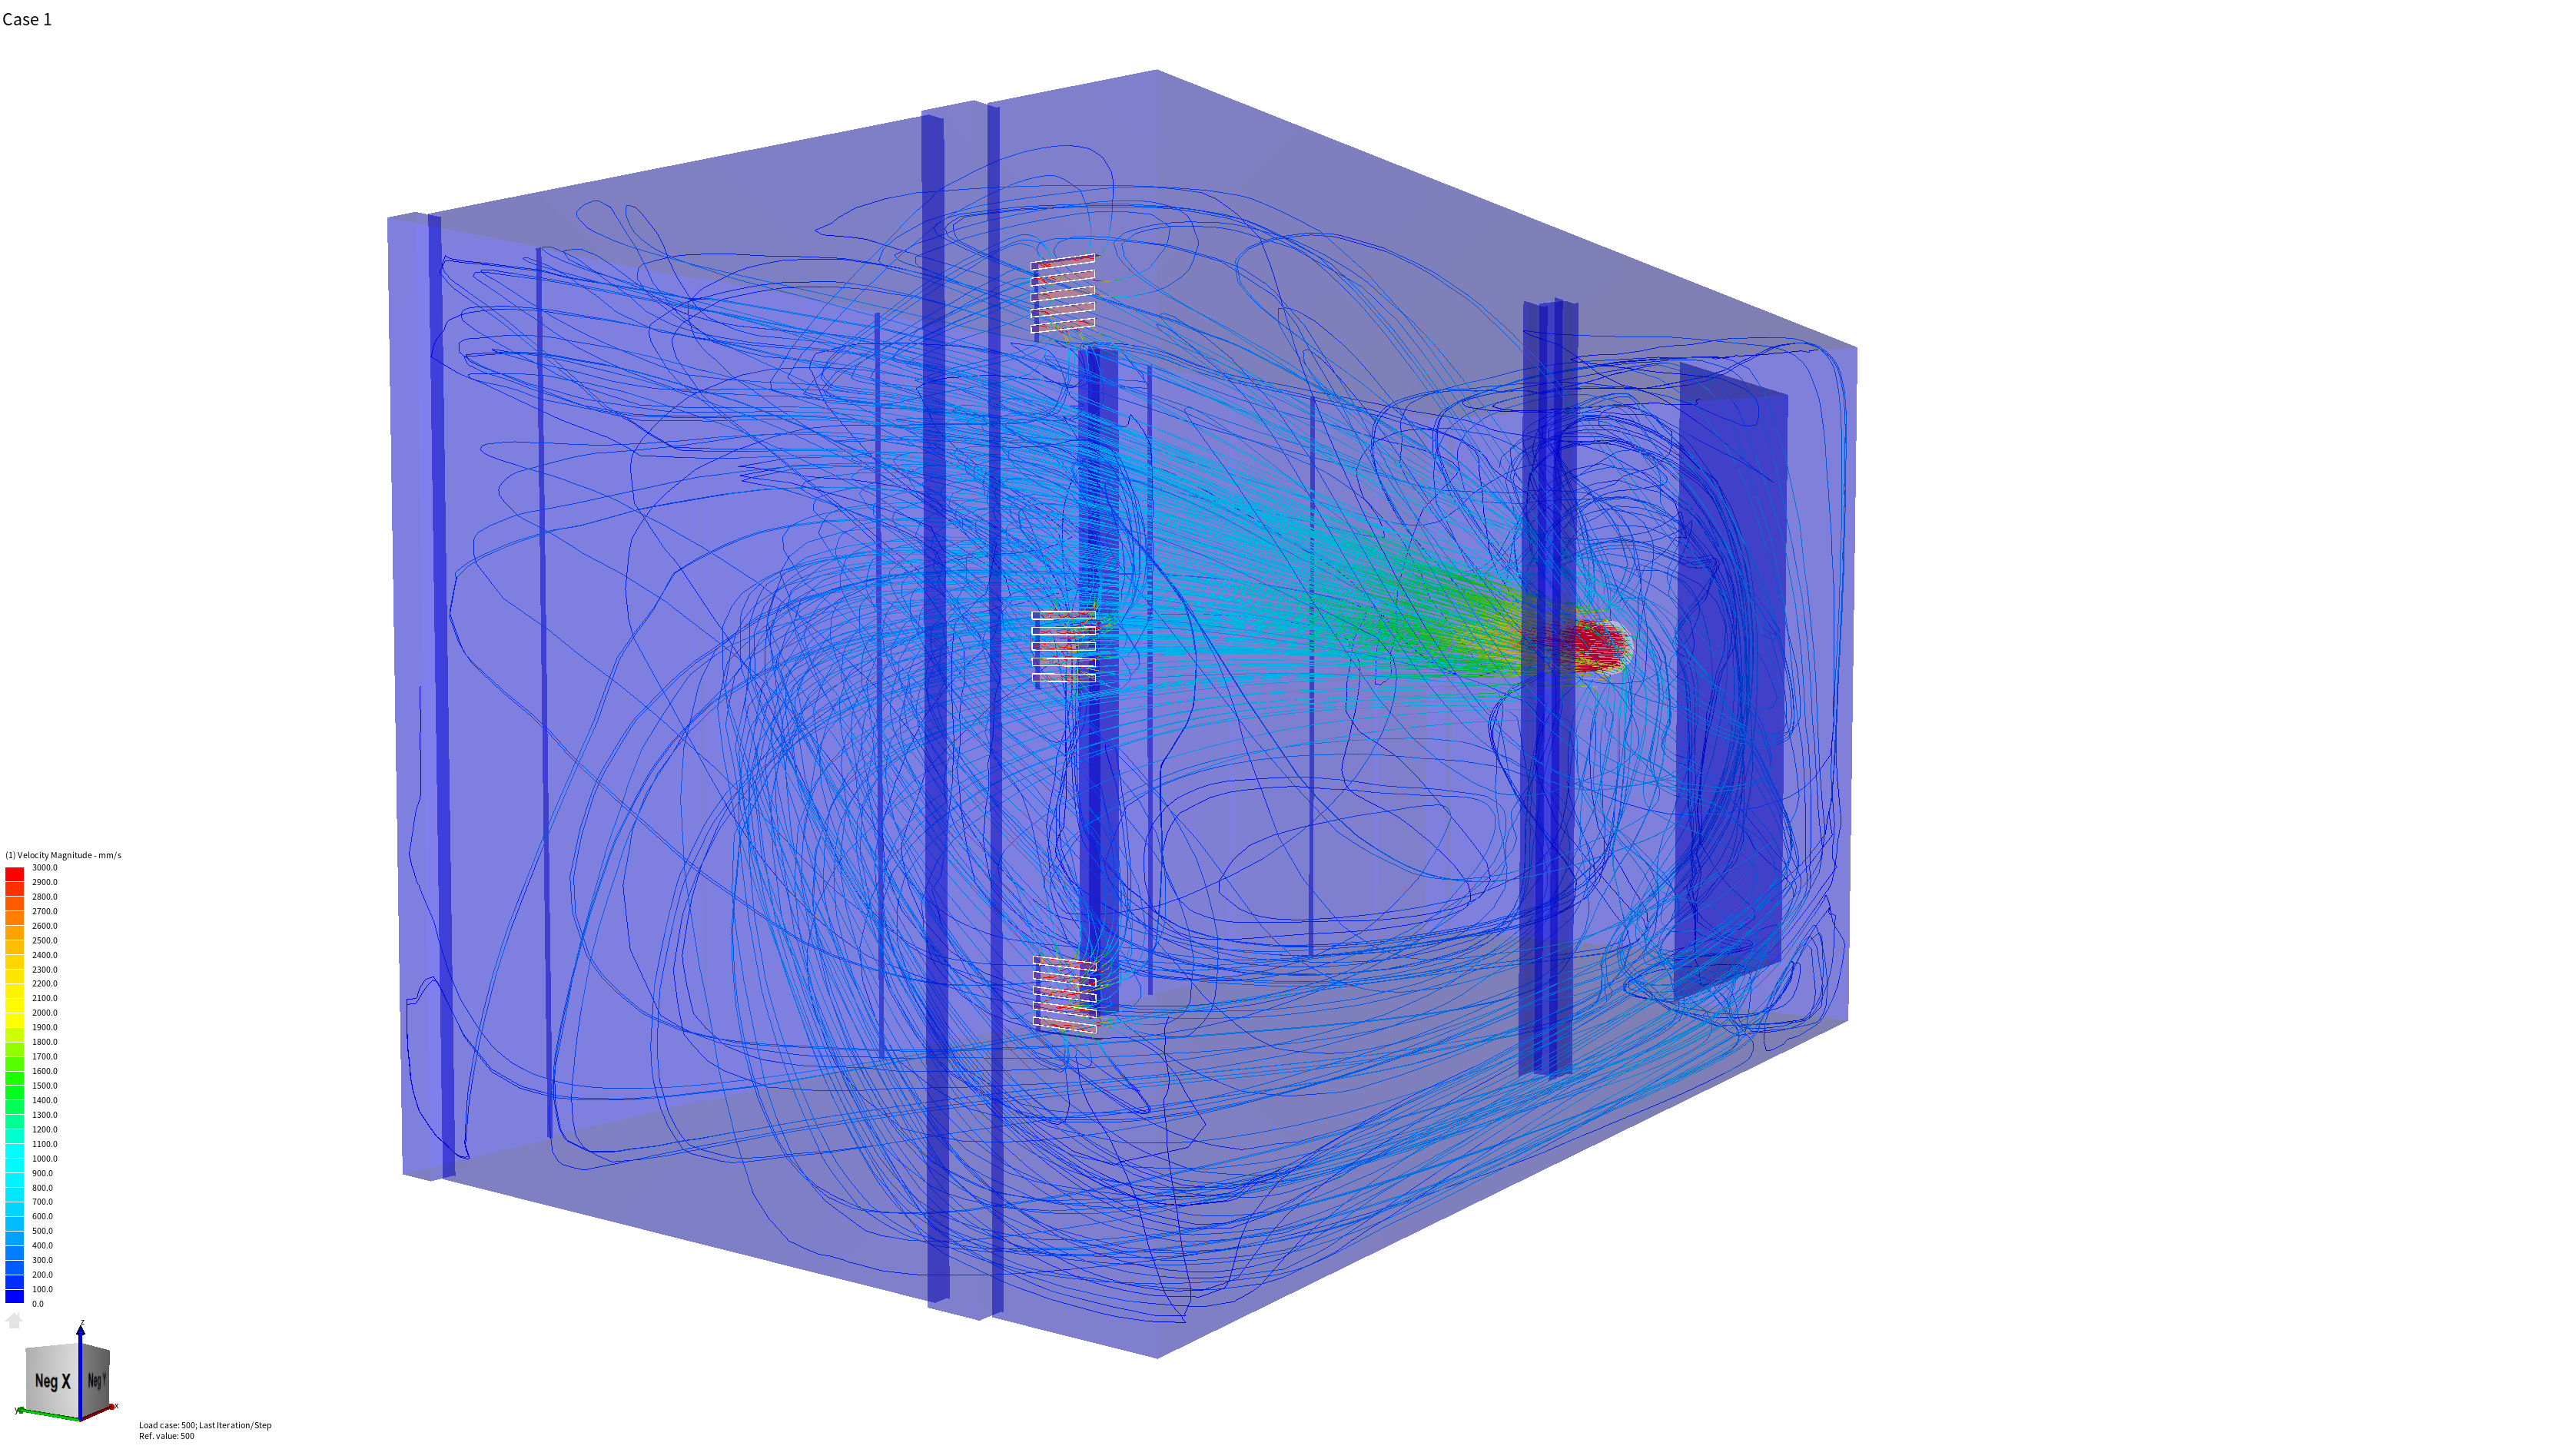
\includegraphics[width=0.92\textwidth]{figures/cfd_streamlines_3d.png}
	\caption{Líneas de corriente coloreadas por magnitud de velocidad. Vista isométrica del recinto; la inyección se localiza en el extremo derecho y la exfiltración se distribuye entre las tres rejillas del lado opuesto. Escala 0--8200~mm/s.}
	\label{fig:cfd_streamlines}
\end{figure}

\begin{figure}[htbp]
	\centering
	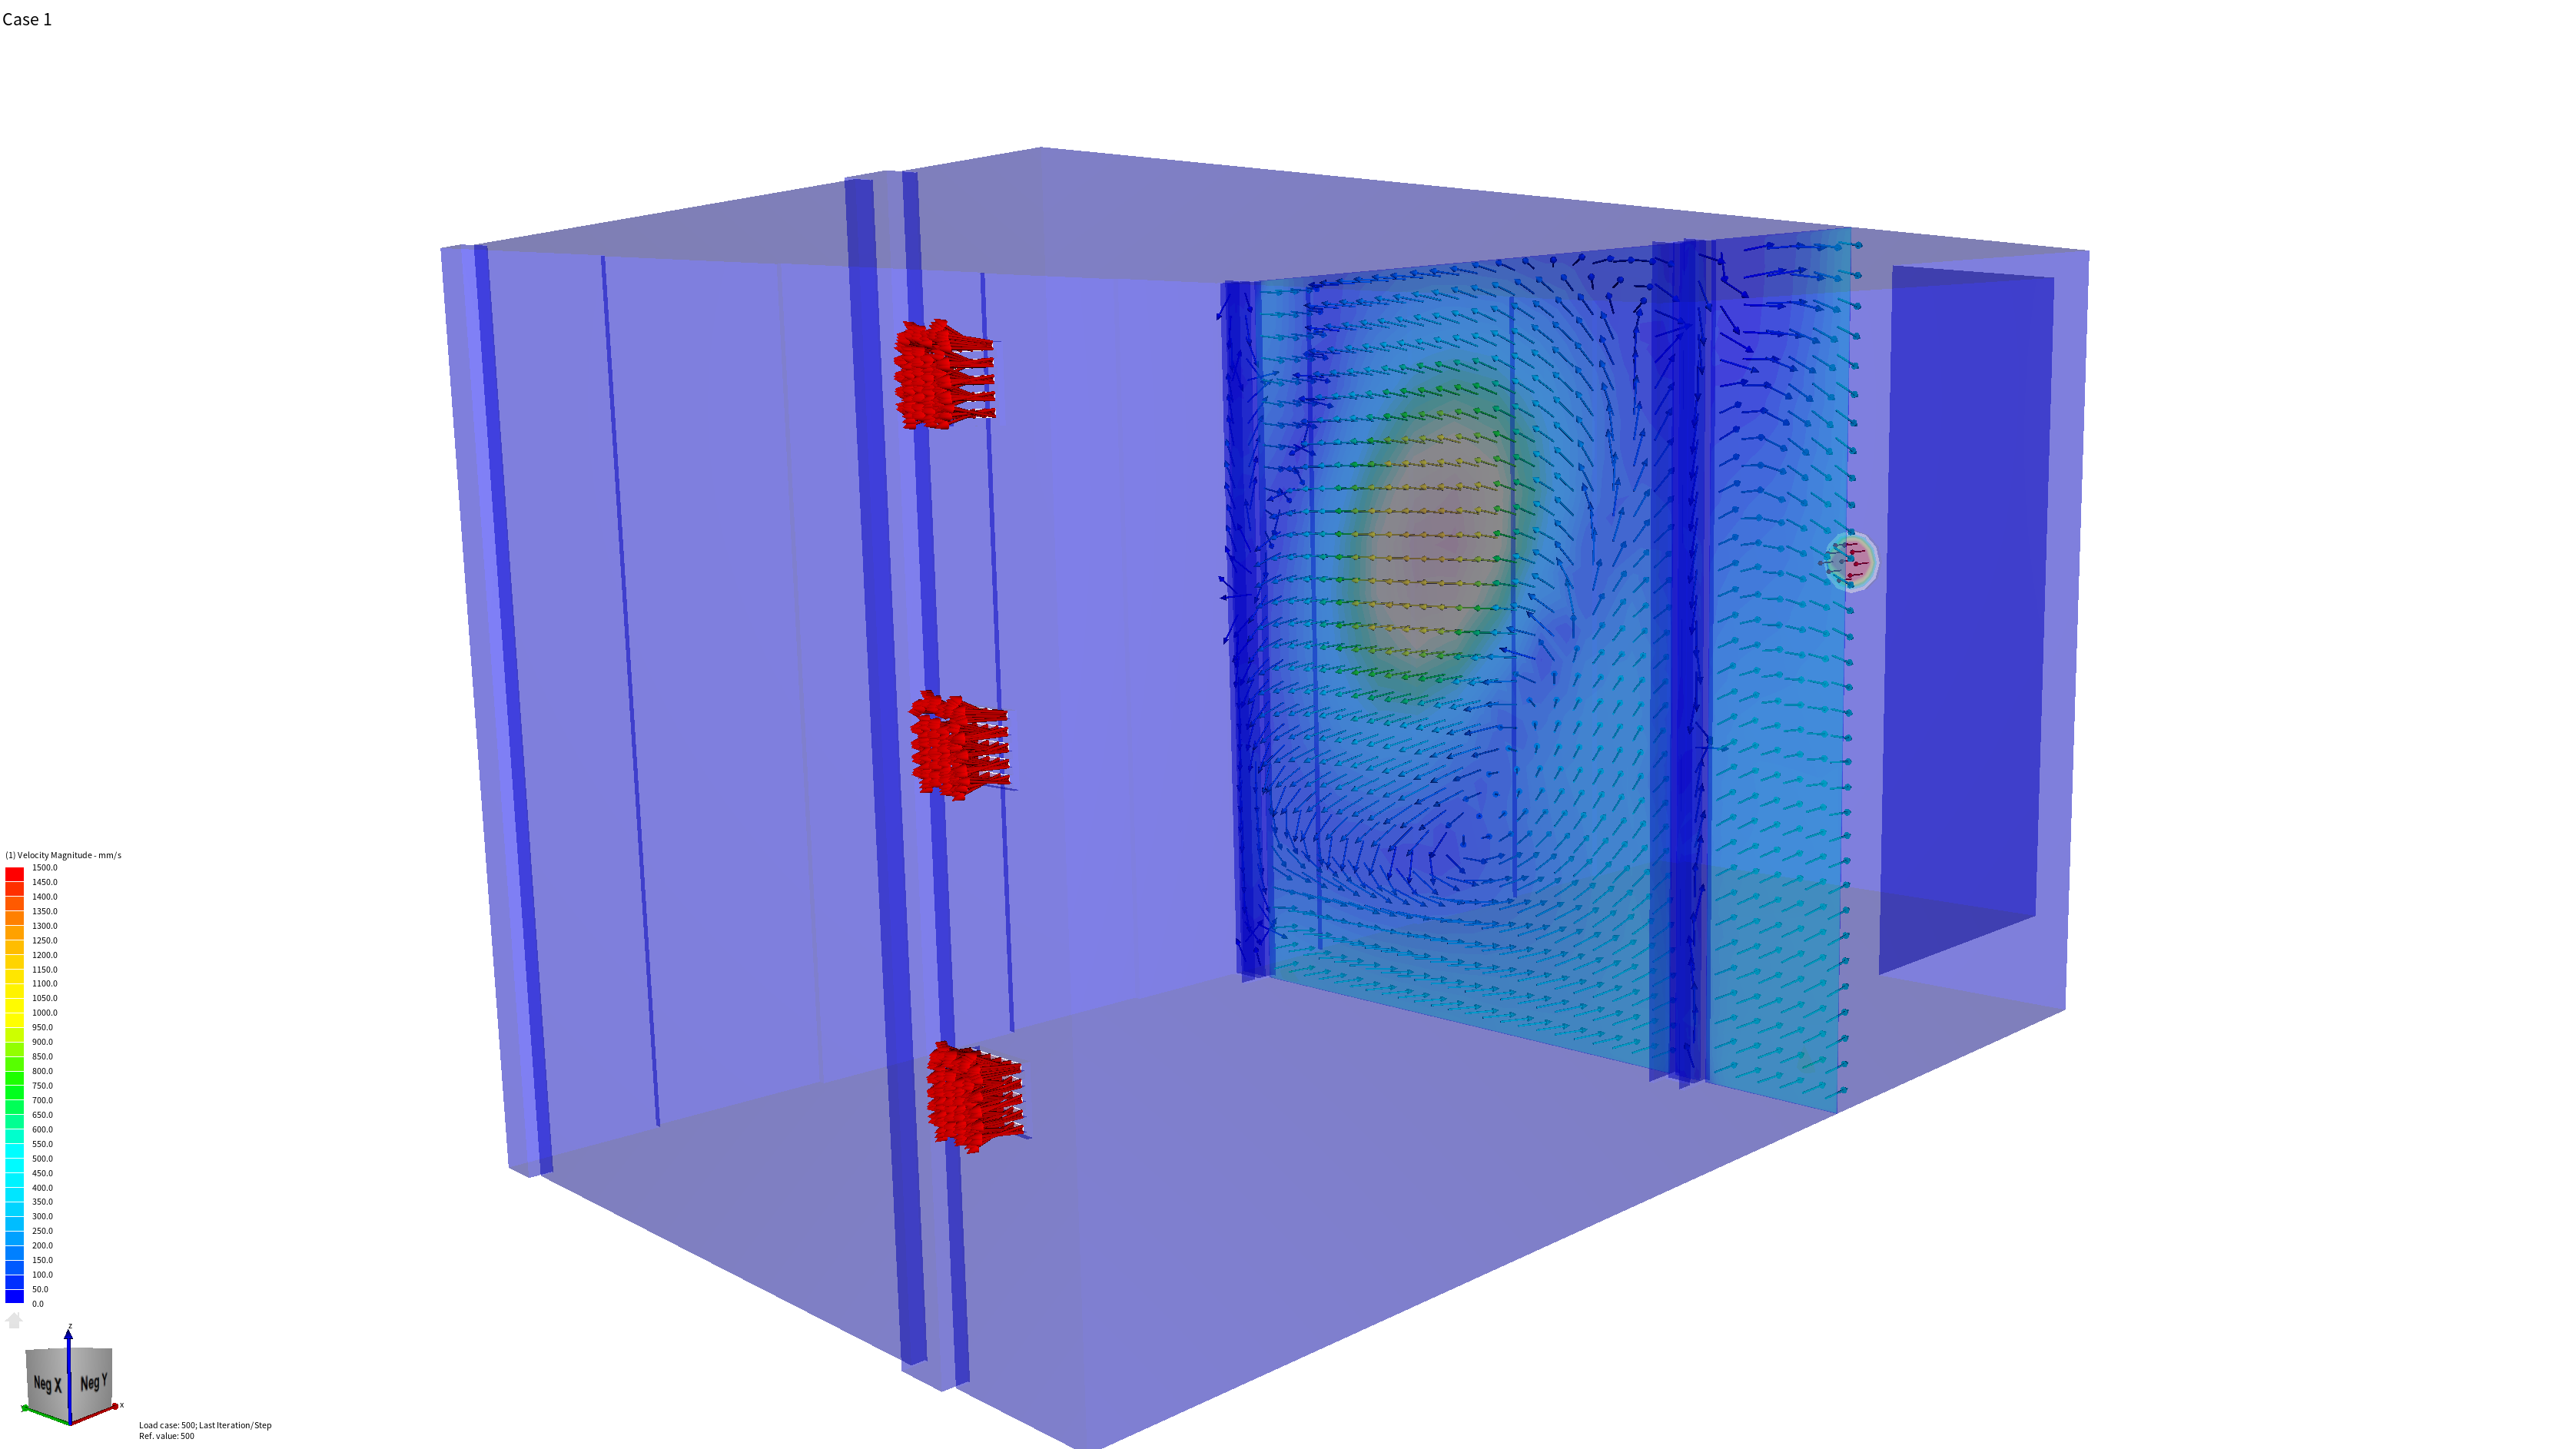
\includegraphics[width=0.92\textwidth]{figures/cfd_vectores_3d.png}
	\caption{Campo vectorial de velocidad en un corte vertical del recinto (vista isométrica). Se observa el flujo dirigido hacia las rejillas de exfiltración y la recirculación en la zona posterior.}
	\label{fig:cfd_vectores_3d}
\end{figure}

\begin{figure}[htbp]
	\centering
	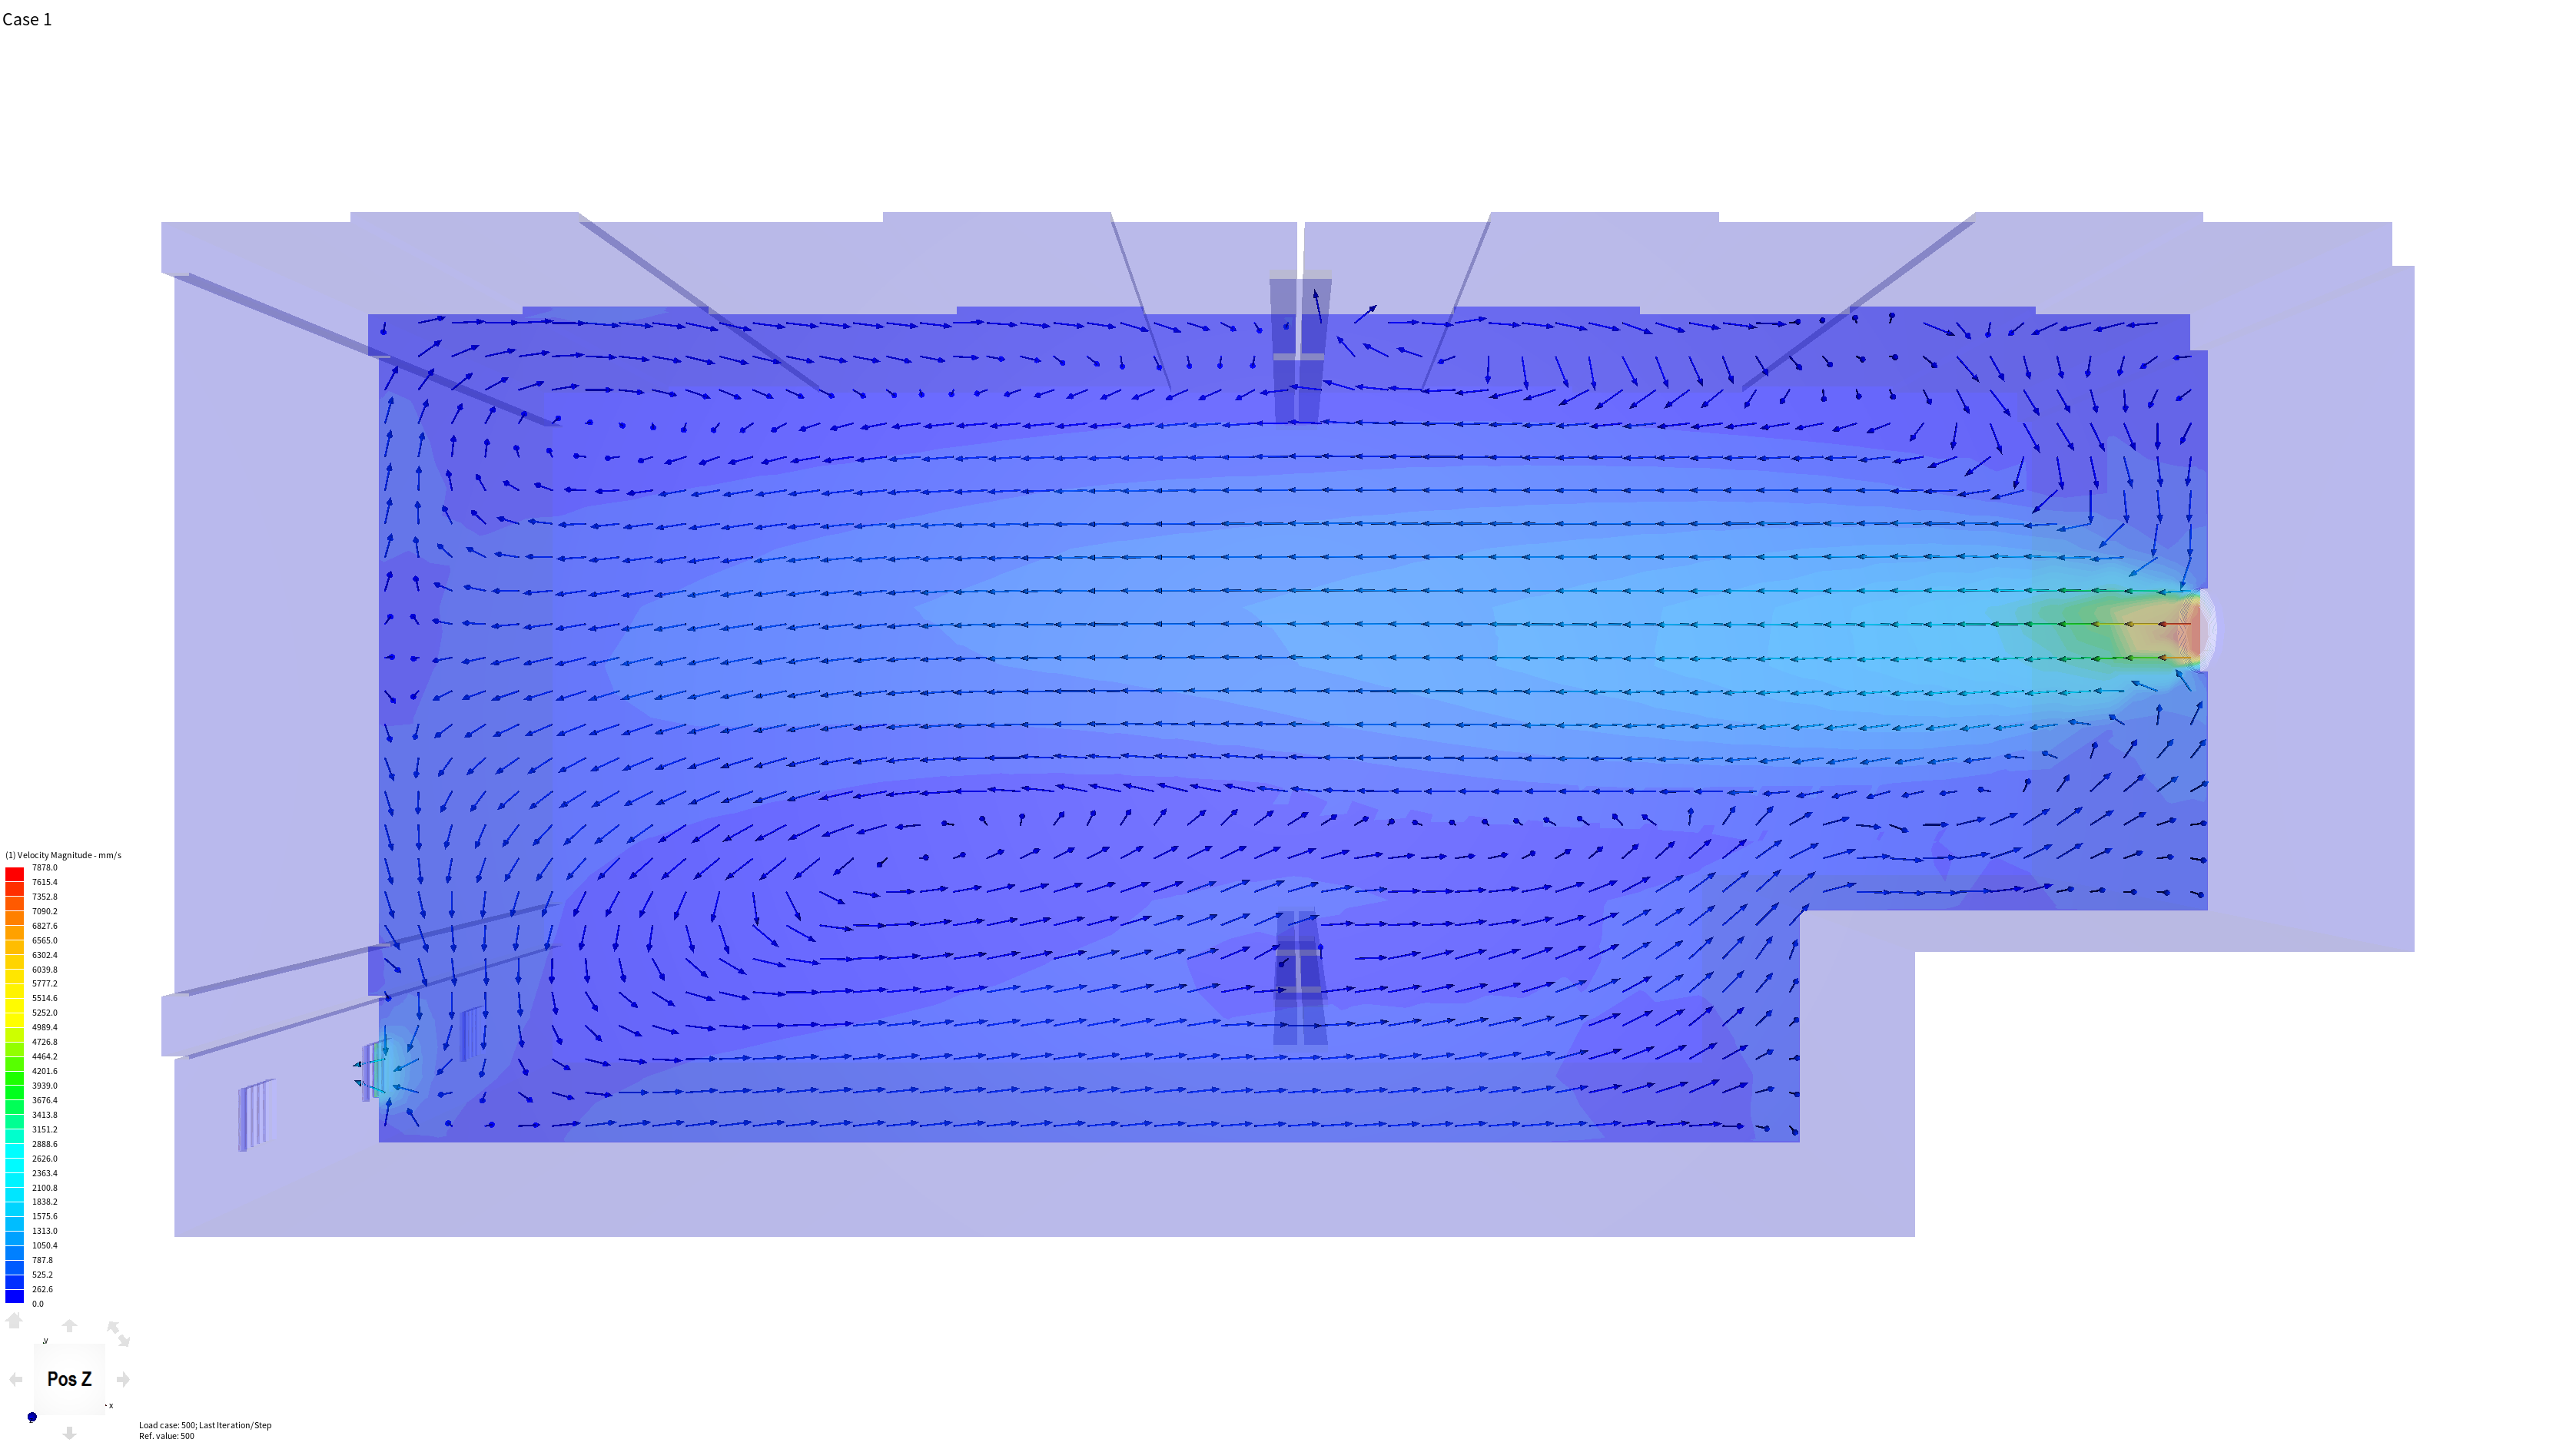
\includegraphics[width=0.92\textwidth]{figures/cfd_planta_horizontal.png}
	\caption{Campo de velocidad en plano horizontal (vista en planta). La inyección desde la derecha genera un flujo cruzado hacia las tres rejillas de la izquierda; las zonas periféricas presentan vórtices de baja velocidad.}
	\label{fig:cfd_planta_horizontal}
\end{figure}

\begin{figure}[htbp]
	\centering
	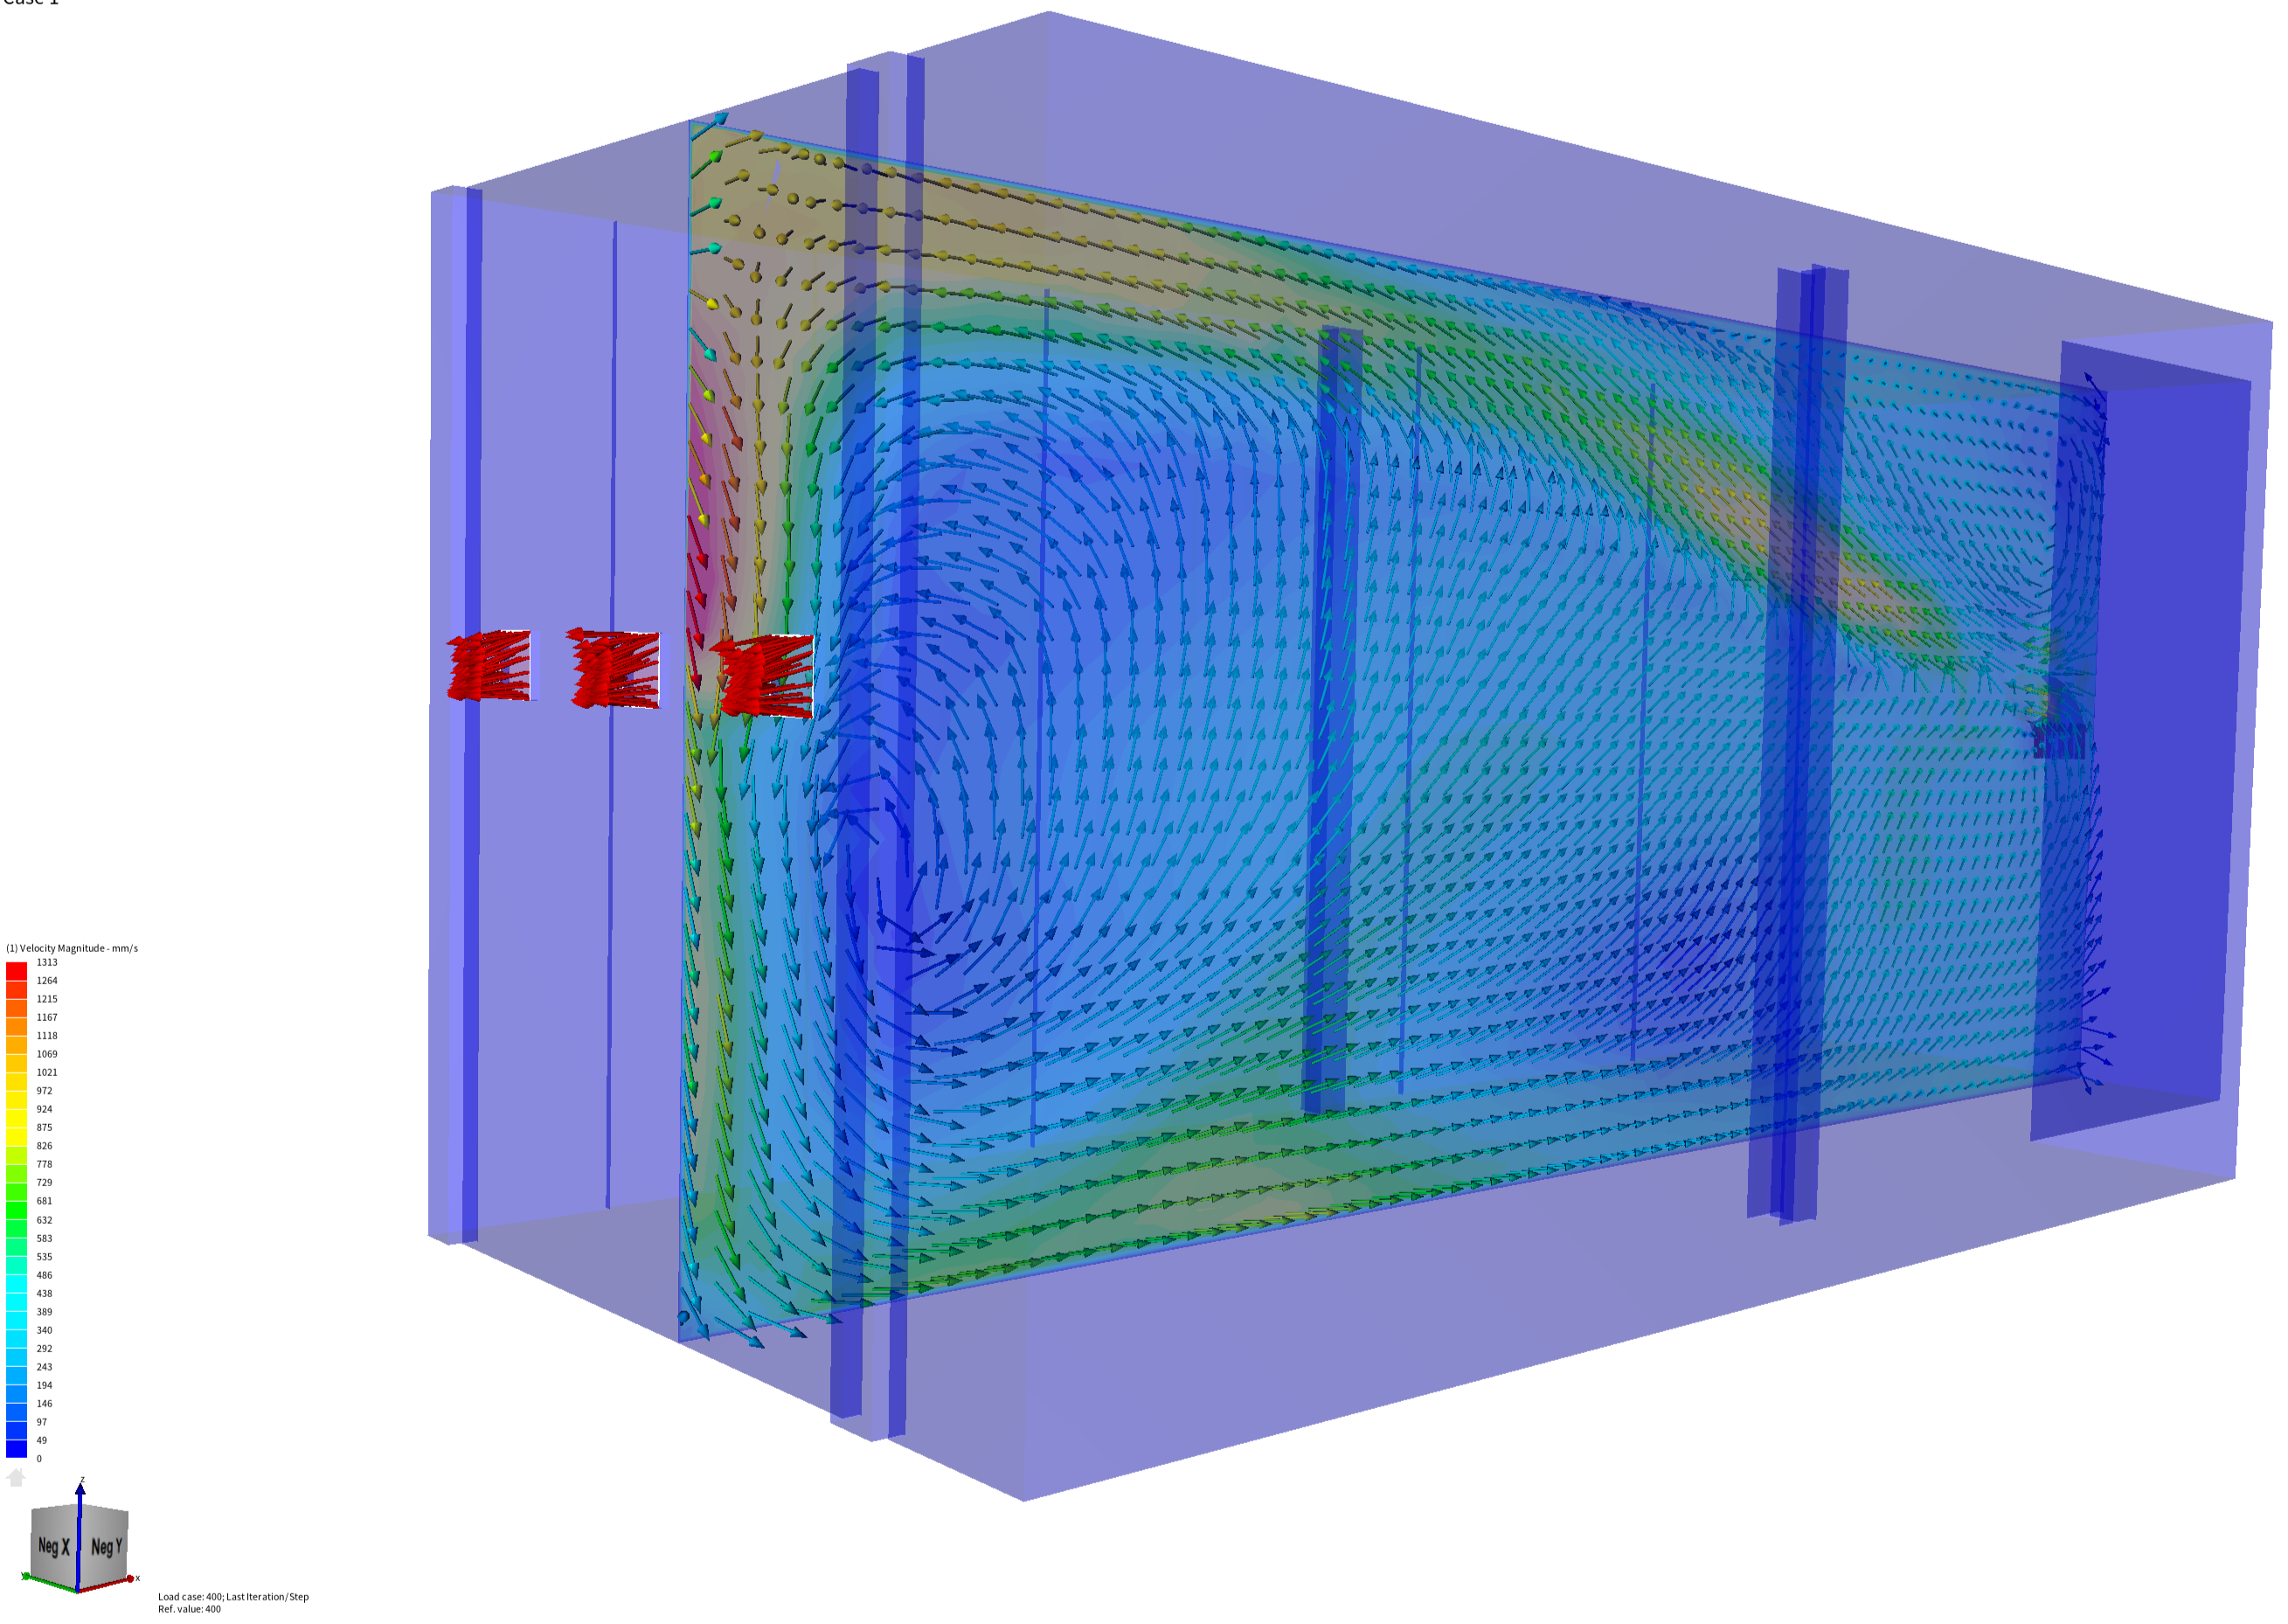
\includegraphics[width=0.92\textwidth]{figures/cfd_vectores_corte.png}
	\caption{Campo vectorial de velocidad en un corte longitudinal. Se aprecia la inyección lateral, la difusión del chorro y el patrón de recirculación en la mitad opuesta del recinto.}
	\label{fig:cfd_vectores_corte}
\end{figure}

\section{Análisis de Resultados}\label{sec:analisis}

Los resultados obtenidos indican que el caudal de diseño de 2 260 CFM satisface el requerimiento de 12 renovaciones de aire por hora para el volumen de 320 m$^3$. Este valor se encuentra dentro de los rangos recomendados por ASHRAE 170 para espacios de laboratorio y por el WHO Laboratory Biosafety Manual para instalaciones BSL-2, con margen de seguridad respecto al mínimo de 6 ACH.

La potencia teórica del ventilador, calculada en 0.320 kW para un escenario de presión total de 165 Pa a las condiciones del sitio (Cajicá, 2 558 msnm, $\rho$ = 0.88 kg/m$^3$), es consistente con el orden de magnitud esperado para un ventilador axial de impulsión de caudal medio en aplicaciones de ventilación de laboratorio. La selección provisional de un motor de 0.75 HP TEFC anticorrosivo proporciona un factor de seguridad adecuado para compensar pérdidas adicionales por ensuciamiento de filtros, variaciones de eficiencia y condiciones de operación no ideales; el valor definitivo se confirmará con la curva de catálogo del axial seleccionado.

La velocidad de impulsión de 8 m/s en la boca del ventilador se ubica dentro del rango recomendado de 6 a 12 m/s para ventiladores centrífugos y axiales de impulsión directa. Esta velocidad permite un ingreso de aire ordenado sin generar ruido excesivo ni corrientes locales molestas en el interior del recinto.

La velocidad de descarga de 3.0 m/s en las rejillas de salida responde a un criterio de confort y de pérdida de presión baja en la descarga libre: una velocidad excesiva aumentaría el ruido y la velocidad del aire en las zonas cercanas a las rejillas. El valor seleccionado se encuentra dentro del rango aceptable de 2.5 a 4.0 m/s para aplicaciones de laboratorio y representa una pérdida de descarga de solo 11 Pa a la densidad del sitio.

La configuración de descarga adoptada, definida por BRINSA, dispone las tres rejillas apiladas verticalmente, una sobre otra, en la pared opuesta a la inyección. Esta disposición concentra las salidas en una sola columna vertical y fue la configuración evaluada en el modelo CFD; como se discute a continuación, la simulación confirma que el caudal se distribuye entre los tres niveles y que no se generan zonas de estancamiento severo.

El modelo CFD, resuelto con salidas tipo \texttt{pressure outlet} a \SI{0}{Pa} gauge (descarga libre a la atmósfera), confirma el comportamiento esperado del sistema de ventilación. Las Figuras \ref{fig:cfd_streamlines} y \ref{fig:cfd_streamlines_b} muestran que el aire inyectado describe un chorro dirigido hacia la pared de descarga, alineado a altura media con la rejilla central de la columna; al aproximarse a la pared opuesta, las líneas de corriente se abren verticalmente para alimentar las rejillas superior e inferior, sin retorno hacia la inyección, lo cual evidencia una distribución de flujo ordenada a través del recinto. La escala de velocidad alcanza aproximadamente \SI{8}{m/s} en la boca de impulsión y desciende progresivamente hacia las salidas.

Las Figuras \ref{fig:cfd_vectores_3d} y \ref{fig:cfd_vectores_3d_b} evidencian en el corte vertical la difusión del chorro y la formación de celdas de recirculación en los tercios superior e inferior del recinto. Aunque existe recirculación, los vectores mantienen dirección de salida en las tres rejillas apiladas, sin indicios de flujo entrante. Esta recirculación es aceptable en un sistema de ventilación por dilución siempre que no genere zonas de estancamiento prolongado; la propia recirculación es el mecanismo que alimenta las rejillas de los extremos de la columna, por lo que contribuye a distribuir el caudal de descarga entre los tres niveles.

Las Figuras \ref{fig:cfd_planta_horizontal} y \ref{fig:cfd_planta_horizontal_b}, correspondientes al corte horizontal a la altura de la rejilla central, confirman el barrido longitudinal entre la pared de inyección y la pared de descarga. Los vectores de mayor módulo se concentran en el eje del chorro, mientras que las zonas periféricas presentan dos vórtices de arrastre simétricos de baja velocidad. Este patrón es típico de una inyección localizada sin ductos de distribución; la magnitud de los vórtices no compromete el objetivo de renovación porque el caudal total (12 ACH) garantiza el reemplazo del aire.

Las Figuras \ref{fig:cfd_vectores_corte} y \ref{fig:cfd_vectores_corte_b} refuerzan las observaciones anteriores en el plano vertical longitudinal que atraviesa la columna de rejillas: el chorro de inyección mantiene su dirección hasta la proximidad de la pared de descarga, alimenta directamente la rejilla central y, mediante las celdas de recirculación superior e inferior, distribuye el resto del caudal hacia las rejillas de los extremos. Las tres rejillas descargan con velocidades faciales del orden de \SI{3}{m/s}, coherentes con el dimensionamiento, y no se observan corrientes de retorno significativas hacia la inyección ni fugas no modeladas. La distribución de velocidad es coherente con el balance de masas teórico y con el objetivo de ventilación por dilución del recinto.

Finalmente, el balance de masas entre la entrada y la salida del recinto se cierra con una discrepancia inferior al 0.1 \%, lo cual valida la coherencia dimensional y cinemática de los datos de contorno propuestos para el CFD.

\section{Conclusiones}

\begin{enumerate}
	\item El caudal de ventilación requerido para alcanzar 12 renovaciones de aire por hora en el laboratorio de 320 m$^3$ es 64.0 m$^3$/min, equivalente a 3 840 m$^3$/h o 2 260 CFM.
	\item La potencia teórica del ventilador es 0.320 kW para una presión total de 165 Pa a las condiciones del sitio (equivalente de catálogo: 225 Pa a densidad estándar) y una eficiencia del 55 \%. Se recomienda provisionalmente un motor de 0.75 HP para incluir márgenes de operación y degradación de filtros, a confirmar con la curva de catálogo del axial seleccionado.
	\item El área de impulsión del ventilador es 0.1333 m$^2$, correspondiente a un diámetro equivalente de 412 mm y un radio de 206.0 mm, con una velocidad de impulsión de 8 m/s.
	\item Las rejillas de descarga se dimensionan en tres unidades de 353 mm $\times$ 336 mm cada una, operando a una velocidad facial de 3.0 m/s en descarga libre a la atmósfera, lo cual mantiene una pérdida de presión baja sin generar ruido excesivo.
	\item El valor de 12 renovaciones de aire por hora se sustenta en ASHRAE 170, WHO Laboratory Biosafety Manual y NIH DRM, cubriendo el rango superior de laboratorios BSL-2 y el umbral inferior de laboratorios BSL-3.
	\item El modelo CFD, resuelto con inyección a \SI{8}{m/s} y salidas tipo \texttt{pressure outlet} a \SI{0}{Pa} gauge (descarga libre a la atmósfera), confirma el campo de velocidades esperado: velocidad máxima de \SI{8}{m/s} en la inyección, velocidades faciales del orden de \SI{3}{m/s} en las rejillas y flujo general de salida sin retornos hacia el interior, lo que evidencia una ventilación efectiva del recinto.
\end{enumerate}

\section{Recomendaciones}

\begin{enumerate}
	\item Instalar un sensor de presión diferencial entre el laboratorio y la zona adyacente, con un set-point de control entre +12.5 Pa y +25 Pa, para garantizar y monitorear la presurización positiva de forma continua.
	\item Filtrar el aire de impulsión con filtros de eficiencia MERV 13-14 (decisión definitiva). El laboratorio es de análisis industrial y no de biocontención, por lo que no se requiere filtración HEPA; los escenarios HEPA evaluados quedan descartados.
	\item Instalar un damper de alivio calibrable como componente obligatorio del lazo de control de presión: a la densidad del sitio (0.88 kg/m$^3$) las rejillas a 3.0 m/s sostienen naturalmente solo 11 Pa, por debajo del mínimo admisible de 12.5 Pa, de modo que el set-point de +25 Pa solo se garantiza modulando la exfiltración con el damper y el sensor de presión diferencial \cite{dml_hd_inst_001,dml_listado_equipos_2026}.
	\item Especificar materiales resistentes al ambiente altamente corrosivo de la planta de hipoclorito de calcio: ventilador, rejillas, damper y soportes en PRFV o acero inoxidable 316, o con recubrimientos epóxicos, y motor TEFC anticorrosivo.
	\item Sellar adecuadamente puertas, ventanas, pasos de instalaciones y cualquier abertura no controlada del recinto, con burletes y umbrales herméticos, para reducir las fugas no controladas y facilitar el mantenimiento de la presión positiva.
	\item Ubicar las tres rejillas de exfiltración en paredes opuestas o perpendiculares a la impulsión, de modo que se favorezca un flujo cruzado que minimice zonas de estancamiento.
	\item Validar la presión diferencial real en campo tras el balanceo y ajuste del damper de alivio, comparándola con el campo de presión obtenido en el modelo CFD. Considerar un estudio de edad del aire o trazadores si se requiere demostrar la eficacia de mezcla en zonas con recirculación.
	\item Prever un margen de sobredimensionamiento del 10 \% al 20 \% entre el caudal de impulsión y cualquier caudal de extracción localizada (campanas, puntos de captación), de modo que la presión positiva general del recinto no se vea comprometida.
\end{enumerate}


% ===================== BIBLIOGRAFÍA =====================
\bibliographystyle{elsarticle-num}
\bibliography{references/bibliografia.bib}

% ===================== ANEXOS =====================
% ===================== ANEXOS =====================
\appendix
\section{Cálculos Detallados}
\label{appendix:calculations}

\subsection{Cálculo del Caudal de Ventilación}

Aplicando la Ec. (\ref{eq:caudal}) con $V = 320$ m$^3$ y $N = 12$ ren/h:

\begin{equation}
	Q = \frac{320 \times 12}{60} = 64.0 \text{ m}^3/\text{min}
\end{equation}

La conversión a m$^3$/h y CFM es:

\begin{equation}
	Q = 64.0 \times 60 = 3\,840 \text{ m}^3/\text{h}
\end{equation}

\begin{equation}
	Q = 64.0 \times 35.3147 = 2\,260.1 \text{ CFM}
\end{equation}

\subsection{Cálculo de la Potencia del Ventilador}

El caudal en unidades SI es:

\begin{equation}
	Q_s = \frac{64.0}{60} = 1.0667 \text{ m}^3/\text{s}
\end{equation}

Para el escenario de diseño con $\Delta P = 190$ Pa (condiciones del sitio, $\rho$ = 0.88 kg/m$^3$) y $\eta = 0.60$:

\begin{equation}
	P = \frac{1.0667 \times 190}{0.60 \times 1000} = 0.338 \text{ kW}
\end{equation}

En unidades de caballos de fuerza:

\begin{equation}
	P = 0.338 \times 1.341 = 0.45 \text{ HP}
\end{equation}

\subsection{Cálculo del Área de Impulsión}

Con $v_{vent} = 8$ m/s:

\begin{equation}
	A_{vent} = \frac{1.0667}{8} = 0.1333 \text{ m}^2
\end{equation}

\begin{equation}
	D = \sqrt{\frac{4 \times 0.1333}{\pi}} = 0.412 \text{ m} = 412 \text{ mm}
\end{equation}

\begin{equation}
	r = \frac{412}{2} = 206.0 \text{ mm}
\end{equation}

\subsection{Cálculo de las Rejillas de Exfiltración}

Con $v_{salida} = 3.0$ m/s:

\begin{equation}
	A_{exfil} = \frac{1.0667}{3.0} = 0.3556 \text{ m}^2
\end{equation}

Para tres rejillas:

\begin{equation}
	A_{rejilla} = \frac{0.3556}{3} = 0.1185 \text{ m}^2
\end{equation}

Seleccionando una relación de aspecto $w/h = 0.95$:

\begin{equation}
	h = \sqrt{\frac{0.1185}{0.95}} = 0.3532 \text{ m} = 353.2 \text{ mm}
\end{equation}

\begin{equation}
	w = \frac{0.1185}{0.3532} = 0.3355 \text{ m} = 335.5 \text{ mm}
\end{equation}

\subsection{Verificación del Balance de Masas}

Caudal de entrada:

\begin{equation}
	Q_{entrada} = A_{vent} \cdot v_{vent} = \frac{Q_s}{v_{vent}} \cdot v_{vent} = Q_s = 1.0667 \text{ m}^3/\text{s}
\end{equation}

Caudal de salida:

\begin{equation}
	Q_{salida} = 3 \cdot A_{rejilla} \cdot v_{salida} = 3 \times 0.1185 \times 3.0 = 1.0665 \text{ m}^3/\text{s}
\end{equation}

La discrepancia entre entrada y salida es 0.02 \%, inferior al 0.1 \%, atribuible al redondeo de dimensiones.

\section{Planos y Esquemas}
\label{appendix:drawings}

Los planos de ubicación del ventilador, rejillas de exfiltración y sensor de presión diferencial se incluirán en una entrega posterior, una vez validada la distribución de flujo mediante el modelo CFD.

\section{Especificaciones Técnicas}
\label{appendix:specs}

Las especificaciones técnicas del ventilador, filtros y rejillas se definirán en la etapa de ingeniería de detalle, con base en los parámetros de diseño entregados en el presente informe.

\section{Documentos de Ingeniería del Proyecto}
\label{appendix:doclist}

Los documentos internos que soportan la investigación y la selección de equipos del sistema de ventilación se listan en la Tabla \ref{tab:project_docs}; todos se conservan en la carpeta \texttt{Investigacion/Sistemas/} del proyecto.

\begin{table}[htbp]
	\centering
	\caption{Documentos de ingeniería del proyecto P2437}
	\label{tab:project_docs}
	\setcounter{itemcount}{0}
	\begin{tabularx}{\textwidth}{@{}NlX@{}}
		\toprule
		\multicolumn{1}{c}{\textbf{Item}} & \textbf{Código} & \textbf{Documento / Propósito} \\
		\midrule
		& -- & Informe de investigación del sistema de ventilación: condiciones del sitio y selección preliminar de equipos \cite{dml_informe_investigacion_2026} \\
		& -- & Listado de equipos y accesorios del sistema (BOQ, 17 ítems) \cite{dml_listado_equipos_2026} \\
		& HD-VENT-001 & Hoja de datos del ventilador de impulsión: centrífugo en PRFV, 3 840 m$^3$/h a 260 Pa (catálogo), motor 1.0 HP TEFC 440 V \cite{dml_hd_vent_001} \\
		& HD-FILT-001 & Hoja de datos del sistema de filtración: prefiltro MERV 8 + filtro V-bank MERV 13-14 \cite{dml_hd_filt_001} \\
		& HD-REJ-001 & Hoja de datos de las rejillas de exfiltración: 3 unidades de 353 mm $\times$ 336 mm, acero inoxidable 316L con malla anti-insectos \cite{dml_hd_rej_001} \\
		& HD-INST-001 & Hoja de datos de los instrumentos de presión diferencial: indicador Magnehelic + transmisor MS-121, set-point +25 Pa \cite{dml_hd_inst_001} \\
		\bottomrule
	\end{tabularx}
\end{table}

	
\end{document}
